This chapter gives describes the theoretical background to estimating the utility of vocabulary.
We first discuss how this work connects to research about vocabulary acquisition for second language learners in Section \ref{sec:context-of-work}.
After this, we define the exact aim of the work in Section \ref{sec:statement-of-goal}.
The following three sections explain the (partially overlapping) fields of Natural Language Processing, Machine Learning, and Explainable AI, tools from all of which are employed in our word utility evaluation approach laid out in Chapter \ref{ch:approach}.
Finally, we examine current approaches for selecting vocabulary for language learners in Section \ref{sec:ranking-lists-of-vocabulary}, to show what methods are currently employed and how they could be improved.


\section{Context of the Work} \label{sec:context-of-work}

This section contextualizes the contents of this work by introducing theoretical considerations by linguistic researchers on the point of vocabulary lists.
This serves to motivate our research, and makes clear what it does and does not aim to achieve, which is explicitly laid out in the second half of the section.


\subsection{Linguistic Motivation} \label{sec:linguistic-motivation}
The issue of which words to learn when setting out to acquire a language is not a new one.
Every textbook on language which does not focus exclusively on grammar must address the issue, and proactive learners will doubtless find themselves looking for ways to optimize the return on their invested studying time.

The Routledge Handbook of Second Language Acquisition \cite{liRoutledgeHandbookSecond2022} is a comprehensive reference work which addresses the various challenges in second language acquisition, including the role of feedback in language learning, the setting for learning and individual differences between learners.
The chapter concerned with vocabulary acquisition gives three criteria for deciding the order in which words are taught to beginners:

\begin{enumerate}
	\item Frequency
	\item Usefulness
	\item Easiness
\end{enumerate}

The first criterion, frequency, is easy to justify:
Learning words that appear with great frequency allows the learner to understand the maximum percentage of words in texts, and should thus be among the most relevant.

Secondly, there is the criterion of "\textit{usefulness}".
While it is acknowledged as a separate criterion from frequency, the authors do not define what constitutes usefulness, or how it might be measured.

The \textit{easiness}, or \textit{learnability} of a word is defined as how easy it is for a learner to acquire the word.
The authors define it with respect to an individual learner since it is posited that the various linguistic backgrounds of learners influence which words they can acquire with ease.
Apart from learner-independent factors influencing the learnability of a word such as word length, whether the learner already knows a cognate of the word will certainly also have an impact:

We can imagine a native German speaker attempting to learn English:
The word "internationalization" may not be a particularly frequent word in most contexts and thus not seem too important to teach, but the German will likely recognize the word as a cognate of the German equivalent "Internationalisierung", and acquire the word with ease, giving a justification for teaching the word early if we wish to impart the most language knowledge as quickly as possible.

In their 2019 paper \cite{heChoosingWordsTeach2019}, He and Godfroid pick up the above three criteria in order to group words into clusters which should help determine their priority in vocabulary learning.
However, again it is not defined what constitutes usefulness and no way to measure it is suggested beyond "human intuition".
In fact, it is put in contrast with frequency, which may be derived from corpus data, whereas usefulness cannot.

It can be seen from the previous examples that a concept of \textit{usefulness} exists in discussions about what the best order in which to teach vocabulary might be, but that it has hitherto not been examined empirically.
The aim of this work is to find ways to evaluate word usefulness, or utility, automatically.
Therefore, the following section defines utility and related concepts more carefully, in order to state the aim of this work more formally.

\subsection{Statement of Goal} \label{sec:statement-of-goal}
Generally speaking, this work addresses the problem of evaluating how useful it is to learn a given word in the target language of a language learner.
This helps us in generating ordered lists of vocabulary to learn which aid the learner in gaining competency in their target language quickly.
Since different language learners learn languages for different reasons, we attempt to take into account the learner's motivation to tailor vocabulary specifically to the individual.
This stands in contrast to traditional learning resources such as textbooks, which, by their linear and static structure, cannot take individual differences in interests of learners into account.
To make this goal more specific, we define several concepts that help us speak more precisely about this goal and how it may be accomplished.
These concepts are used throughout this work.

\subsubsection{Linguistic Context}
The ways in which people interact with language (a "context") can be described from many different perspectives and along different dimensions, such as the level of formality, the topic or the setting of the interaction.
In this work, a \textit{linguistic context} or just \textit{context} refers to one particular such way of linguistic interaction.
Examples of language contexts by topic are:
News, football, crocheting.
Examples of language contexts by situation are:
Everyday conversation, scientific articles, watching movies.
Contexts can be further subdivided into smaller contexts, or grouped across different lines:
"News" could be subdivided into "international politics", "sports", "business", etc.

The concept of a language context is useful to a language learner since it enables them to prioritize learning vocabulary and grammar associated with the context they are interested in:
Someone who is learning Arabic to better understand middle-eastern politics will have little use for words which are mostly associated with football.

The context can even determine the length and complexity of sentences that a learner must be able to understand:
We will see in Section \ref{sec:final-dataset} that sentence in Wikipedia articles are about three times longer, on average, that those found in movie subtitles.
Thus, learning for one or multiple specific contexts gives the learner a more concrete goal and thus better idea of what they must learn to achieve it.

In contemporary methods and tools for language learning, usually little emphasis is placed on learning for a specific context.
This is partially due to the format of these tools:
A static resource, such as a textbook, cannot cater to individual preferences of learners.
Some publisher produce books on "Business English" or "Technical English", but each of these take manual effort to produce and can hence address only a few, relatively broad contexts, in addition to being scarce for less studied languages:
For instance, despite being the 21st most spoken language in the world
\footnote{According to the Encyclopedia Britannica \url{https://www.britannica.com/topic/languages-by-total-number-of-speakers-2228881}, last accessed April 22, 2025}
, no textbook on Business Vietnamese is sold by any major US publisher such as Pears \footnote{\url{https://www.pearson.com}}, HMH \footnote{\url{https://www.hmhco.com}}, or McGraw Hill \footnote{\url{https://www.mheducation.com}}.
Classroom lectures, where groups of students are taught in one course, can also only cater to individual preferences to a limited degree, especially if they are oriented around textbooks, for the above reason.
In this work, we will present an approach for the compilation of context-specific vocabulary lists that requires minimal effort to expand to new languages or contexts.

\subsubsection{Utility} \label{sec:utility}
In this work, the \textit{utility} of a word is defined as the increase of language ability in a given context that a person gains by knowing a word versus not knowing it at all.
Here, language ability refers to being able to understand more of texts they read in the given context, being able to speak about the subject, etc.
It is easy to see that some words will be more useful than others given a context:
In the context of international news, learning the word "war" will bring more understanding to the learner than "pear" or "polymorphism".

\subsubsection{Proxy Task}
Some of the concepts in the realm of language learning cannot be measured directly:
This can be because they are psychological in nature ("understanding") or because they are too complex to be objectively measured by numbers ("language ability").
The above section defines word utility as an increase in "language ability", but to analyze this ability with computers, we must make be able to put a number on it, even though we lack both an agreed upon scale and unit of measurement.

To circumvent this issue, we use \textit{proxy tasks}:
In this paper, we use the term \textit{proxy tasks} for tasks that test subjects (either human or AI models) can perform, where the test result (the \textit{proxy measure}) is used to capture the abstract quantity under study.
For example, as a proxy measure for a person's general spelling ability, we could make them choose from multiple spelling variants of a word, and use the accuracy with which they select the correct answers.
This work employs AI models solving NLP tasks as an economic and repeatable substitute for real humans interacting with language, and uses the NLP tasks as proxy tasks to make "language understanding", and thus "utility", measurable concepts that can be computationally maximized.

\subsubsection{Revised Statement of Aim}
With the concepts above defined more precisely, we can state the goal more accurately, namely, creating computational methods which can find words that have the maximum \textit{utility} given a particular \textit{language context} by means of \textit{proxy tasks}.
With the words in cursive filled in, this translates to:
Finding words that provide a language learner with the most language understanding in the specific situations they are interested in, requiring them to learn the least possible amount of words.
Since the understanding of a learner cannot be directly measured, we use tasks that check the learner's understanding as an imperfect but necessary approximation.
The following sections discuss the fields addressed in achieving this aim, and highlight relevant aspects from them that contribute in later chapters to conceptualizing and implementing a solution.


\section{Natural Language Processing} \label{sec:natural-language-processing}
While the aim of the work is to develop methods to automatically compile vocabulary lists that serve human learners, the technical implementation of this necessarily will process human language with the use of computers.
This domain is called \textit{Natural Language Processing}, a field defined in The Handbook of Computational Linguistics and Natural Language Processing as the engineering domain of Computational Linguistics \cite{alexanderclarkHandbookComputationalLinguistics2010}.
Natural Language Processing, often abbreviated as \textit{NLP}, is both used in Computational Linguistics (the field concerned with analyzing natural language through language data) and as well as in practical applications such as Chatbots, Machine Translation, Speech Recognition etc. \cite{jurafskySpeechLanguageProcessing2025}.
This work addresses both aspects, as it is an undertaking of Computational Linguistics through the analysis of how AI models perform typical \textbf{NLP tasks}.

\subsection{Corpus}
The typical way Computational Linguistics empirically analyzes language is through the use of \textbf{corpora}.
A common definition of a corpus can be seen in \cite{hunstonCorpusLinguistics2006a} as "an electronically stored collection of samples of naturally occurring language", which "can be a test bed for hypotheses and can be used to add a quantitative dimension to many linguistic studies".

Recently, many large corpora have been compiled and are freely available to the public.
Corpora differ from each other mostly in their source and method of compilation.
Depending on their source, some corpora may serve as examples of language being used in a language context, such as news or movie subtitles.
The idea of using context-specific corpora to compile context-specific vocabulary lists has been used in the past, especially to create lists of academic vocabulary for specific academic fields \cite{xodabandeDevelopingValidatingMidfrequency2023} \cite{gholaminejadAcademicVocabularyCollocations2020}.
In the implementation and evaluation of this work's approach to word utility estimation, we use several such context-specific corpora, as they present a way to analyze how language (and more specifically, vocabulary) is used in the linguistic context of the corpus.

\subsection{NLP Task}
This work attempts to make use of not only static data in the form of corpora, but also the interaction of AI models with those corpora in order to gain insights into word utility.
This active part of \NLP\ consists of performing \textbf{NLP tasks}.
Typical NLP tasks include \cite{jurafskySpeechLanguageProcessing2025}

\begin{itemize}
	\item Sentiment Detection: Given a text, estimate the emotional state of the author.
	\item Masked Language Modeling: Given a text with a word blanked out, estimate what the word should be.
	\item Machine Translation: Given a text, translate it another language while preserving meaning as faithfully as possible.
\end{itemize}

Humans are not trained from childhood to do any one language "task":
They can have conversations, answer questions about things they have seen, etc.
In contrast, the interaction of computers is usually more rigidly defined by specific NLP tasks, and AI models are trained to perform one or several of these tasks.

For the purposes of this work, an \textit{NLP task} is a function with a specific input and output format, where at least one of the two formats takes the form of natural language.
We utilize NLP tasks as a way for AI models to interact with natural language, enabling us to analyze how certain words influence this interaction; the exact approach is described in Chapter \ref{ch:approach}.


\subsection{NLP Pre-Processing: Tokenization} \label{sec:tokenization}
Language presents itself in continuous form in most situations:
When listening to spoken language, it is not obvious where one word ends and another begins.
Likewise, written texts we find online or in books are not necessarily subdivided into its semantic constituents.
While words in the written English language are mostly separated by spaces, a writer may choose to create a new hyphenated word sequence on the spot as necessity demands.

Further complicating the issue of where to separate words is the fact that many non-European languages do not use spaces in their spelling (e.g. Japanese, Mandarin Chinese) or use spaces for a different purpose (separating syllables in Vietnamese, separating sentences in Thai).
For these reasons, \textit{tokenizers} are used in Natural Language Processing to divide continuous texts into individual words \cite{jurafskySpeechLanguageProcessing2025}.


Splitting continuous text into distinct words serves following purposes in this work:
\begin{itemize}
	\item Making statistics from word counts (e.g., counting which words occur many times).
	\item Assigning estimated utility to words.
	\item Being able to remove individual words in text inputs to AI models, in order to test what effect removing a particular word has on the output.
\end{itemize}

Speaking more precisely, tokenizers divide texts into \textit{tokens}, which do not necessarily correspond to words \cite{jurafskySpeechLanguageProcessing2025}:
For instance, the \texttt{bert-base-uncased} tokenizer used in this work splits the word \texttt{enmity} into the sub-word tokens \texttt{en} and \texttt{\#\#mity} (sub-word tokens which are not the start of a word begin with \texttt{\#\#} in their text representation for BERT tokenizers).
As we are interested in counting complete words, we must therefore merge sub-word tokens back into complete words when they occur in our data pipeline.
The details of this are discussed when presenting our implementation in Chapter \ref{ch:implementation}.
In order to provide utility evaluation for words in a wide range of languages, this work employs tokenizers which can handle language of different syntactic structures, and where the tokenizer outputs sub-word tokens, we usually merge the tokens into complete words.

\subsection{NLP Pre-Processing: Named Entity Recognition}
In this work, we attempt to compile lists of vocabulary by processing corpora with various methods.
However, these corpora contain some words which are typically not desirable in vocabulary lists, such as the names of people, organizations, and places.
For this reason, we employ Named Entity Recognition \cite{jurafskySpeechLanguageProcessing2025} (\textit{NER} for short) to handle such words in our approach, and prevent them from appearing in our generate vocabulary lists.
A named entity can be defined "anything that can be referred to with a proper name" \cite{jurafskySpeechLanguageProcessing2025}.
Consider the following sentence:

\begin{quote}
	\textit{Angela Merkel, the chancellor of Germany, visited Karlsruhe last month.}
\end{quote}

This sentence contains the personal name \textit{Angela Merkel}, the country name \textit{Germany} and the city name \textit{Karlsruhe}.
Because personal names such as \textit{Angela Merkel} are generally not seen as vocabulary to learn, when we compile a list of English vocabulary from a corpus containing the above sentences, we filter such names from the lists.
The names of places can be useful vocabulary, such as in the case of \textit{Germany}, because it differs between English and other languages (e.g., German: \textit{Deutschland}, Spanish: \textit{Alemania}).
However, our tool for Named Entity Recognition cannot distinguish between the names of countries and other places such as \textit{Karlsruhe}.
To prevent the vocabulary lists from containing many names of cities, we therefore filter out all recognized names of places, including those of countries.
This is similar to the filtering of named entities performed in the KELLY project \cite{kokkinakisCorpusbasedApproachesCreation2011}:
In it, NER was employed to filter out proper names from its lists of vocabulary.
The only named entities allowed were the names of countries, which were manually added back into the lists after the automatic filtering.


The domain of \NLP\ has in the past been dominated by rule-based methods for processing language.
However, natural language is a very complex subject which is not easily captured by a priori rules \cite{jurafskySpeechLanguageProcessing2025a}.
For this reason, methods based on statistical reasoning on large amounts of linguistic data handle many problems better than manually fixed rules.
Beyond statistical methods, still further advances have been made in the field of Natural Language Processing through the use of AI models such as Neural Networks \cite{jurafskySpeechLanguageProcessing2025a}.
In order to exploit the state-of-the-art tools from the realm of \NLP, this work makes extensive use of such AI models, and therefore the next section therefore briefly introduces the field of Artificial Intelligence.

\section{Artificial Intelligence}
Elaine Rich, in her 1983 work "Artificial Intelligence", defines \AI\ as "the study of how to make computers do things at which, at the moment, people are better" \cite{rich1983artificial}.
An introductory article by IBM describes it as "a technology that enables computers and machines to simulate human learning, comprehension, problem-solving, decision-making, creativity and autonomy"\footnote{\url{https://www.ibm.com/think/topics/artificial-intelligence}, last accessed February 26th, 2025}.
This is opposed to traditional algorithms which can only follow algorithms which have been explicitly programmed.

\subsection{AI Models}
The building block of Artificial Intelligence is called an \textbf{AI Model}, which is a model using training data to learn patterns, and then used on inputs that were not identically present in the training dataset.
AI models are used in this work to simulate an agent interacting with language.
The (pre-trained) AI model is thought of as a test subject in possession of linguistic skills that can be studied.
Through its training process, AI models learn patterns that are generalizable across the problem domain.
If these patterns resemble the knowledge that humans gain when they learn a new ability, it may be possible to analyze the interaction of AI models with data so that a human learner can learn from their behavior, similar to how humans can observe experts in their domain and learn from their behavior.
The field which provides these methods of analysis is Explainable AI, which is explained in Section \ref{sec:explainable-ai}.

The current de facto standard for recent AI models is the \textit{Neural Network} architecture \cite{jurafskySpeechLanguageProcessing2025}, which attempts to imitate the neural makeup of the human brain.
Such models achieve state-of-the-art results on most NLP tasks \cite{jurafskySpeechLanguageProcessing2025a}, and all models used in this work are Neural Networks for this reason.
However, within this architecture there exist further subtypes of AI models, the most important for this work is the \textbf{transformer model}.


\subsection{Transformer Model} \label{sec:transformer}
Since their invention in 2017 \cite{vaswani2017attention}, transformer models have brought impressive gains in performance to many fields, including \NLP.
They are a particular type of deep neural network characterized by a mechanism called \textit{attention}.
This chapter briefly introduces this mechanism and how it is used in this work as one way to assign utility to words.

Typically, a transformer model features an encoder and decoder, each of which consist of an attention layer and feed-forward (i.e, non-recursive) neural network.
Figure \ref{fig:transformer-architecture} shows the transformer architecture (featuring both an encoder and decoder).
Due to their lack of recursion seen in networks such as LSTMs and GRUs, transformers are highly parallelizable.

The encoder consists of a so-called \textit{self-attention} layer and a feed-forward neural network.
The self-attention layer assigns weights to relationships between tokens, which contain information about how much the tokens are related to one another.
This information helps the transformers to "focus" on important tokens, or important relationships between tokens.
For generative transformers, there is also a decoder, which takes as inputs the outputs from the encoder network.
It then uses another attention layer (using \textit{cross-attention}) to assign weights to the embeddings before feeding them into another feed-forward network.

Many transformers feature a mechanism called \textit{multi-head} attention.
This means that the relationships between tokens are given weights from multiple \textit{heads}.
These individual heads "learn to perform different tasks", the combination of which helps create a more nuanced understanding of the token relationships \cite{vaswani2017attention}.
Attention is one possible way to attribute importance to inputs \cite{liUnderstandingNeuralNetworks2017}, and thus utility to words in our case.
How exactly this proxy metric is calculated is discussed in Section \ref{sec:xai-methods}.


\begin{figure}[H]
	\centering
	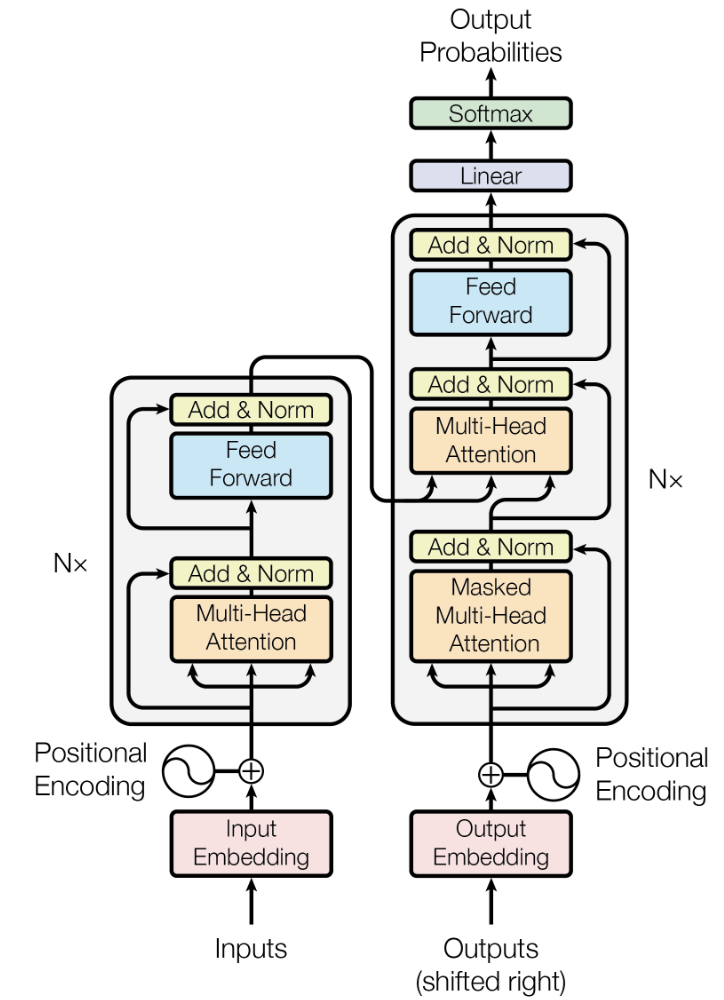
\includegraphics[width=0.5\textwidth]{transformer_architecture.png}
	\caption{The Transformer Architecture. (Source: \textit{Attention is All You Need} \cite{vaswani2017attention})}
	\label{fig:transformer-architecture}
\end{figure}



\subsection{Summary}
This section has introduced the important AI models used in this thesis, namely the Neural Network and one of its most effective subtypes, the transformer.
While these types of AI model have driven many recent improvements in performing common NLP tasks, deep neural networks stop being readily understandable to humans rather quickly once the number of neurons and layers is increased.
We are interested in how the inputs (words) influence the outputs of AI models when performing NLP tasks.
This kind of analysis is the domain of \textbf{Explainable AI}, which is why the next section briefly introduces this last necessary field for the approach put forward in this work.

\section{Explainable AI} \label{sec:explainable-ai}
Explainable AI (abbreviated: XAI) is the fields of research focused on making the decision-making progress of AI models more transparent and understandable to humans, to enable us to reason about the AI model's decisions \cite{viloneNotionsExplainabilityEvaluation2021}.
This can be useful to check if the decision process contains social biases, or if it is based on wrong patterns learned from skewed training and test data (overfitting).
By analyzing the decision process of high-performing AI models, this work attempts to extract useful information about how the language is processed by them which may be useful to humans as well.
For this analysis, XAI is used as a tool to find out which inputs influence the performance of AI models the most.
This section therefore first introduces important distinctions between XAI methods, and argues which types should be used for our purpose.
The result of this evaluation can be seen in Table \ref{table:XAi-method-criteria}.

\subsection{Distinctions between XAI Methods}
There are several categories of XAI methods that are relevant in this work, because they determine not only the purpose of the method, but also which XAI method can be used on which AI model.
This section introduces some of the distinctions and argue why some types are more appropriate to the aim of this thesis than others.

As was mentioned before, this work is interested in analyzing the influence of words in AI model input on its output for the purpose of finding out which words might be the most useful for human learners as well.
The question of which inputs are the most important for a model to reach its output is the domain of \textbf{feature importance explanations}, a sub-field of XAI concerned with "ranking the features by importance" \cite{molnarChapter4Methods2025}.
Thus, all XAI methods in this work belong to this group.

Feature importance explanations can be further subdivided into two groups:
\textbf{Feature selection} methods explain the model's decisions by trying to predict a subset of all input features which are deemed "important".
\textbf{Feature attribution} methods attribute a concrete importance score $a_i$ $\in \mathbb{R}$ to each input feature $x_i$.
This work uses feature attribution methods exclusively, as the scores allow us to rank words in a list by their importance.

Another important characteristics of an XAI method is whether it is \textbf{model-agnostic} or \textbf{model-specific}.
A model-agnostic XAI method can be used no matter what AI model is used, whereas a model-specific method is limited to being used to a specific type of AI model, such as transformers, decision trees, or neural networks.
Model-agnostic models do not look inside the model (e.g., they do not examine weights in neural networks) but only perturb the inputs and observe changes in the model output.
An advantage of model agnostic explanations is that they can be used on any AI model
However, many recent state-of-the-art AI models are built using the transformer architecture, hence methods specific to transformer models can also be fairly broadly applied.
A major upshot of model-specific explanations is their efficiency:
Model-agnostic approaches require us to perturb the input to observe differences in the output, and thus to run the model multiple times for a single explanation, which can constitute a great computational effort.
On the other hand, model-specific methods typically only require one run of the model, as they can look into the model itself for an explanation.
For these reasons, both model-agnostic and model-specific approaches are used in this work.

Another feature of XAI methods is the scope of its explanations:
\textbf{Local} XAI methods explain why a model output was generated for one particular input.
A \textbf{global} method attempts to reason about the model's behavior in general, independent of any particular input data.
This work is interested in observing the interaction of the AI model with a particular corpus, not only the AI model.
For this reason, all methods used in this work are local methods.
However, while local explanations only explain a single decision of the model (which, in the work, is the interaction of the model with a single sentence), we aggregate the individual decisions across the corpus to gain a bigger picture about this interaction.

The transformer attention mechanism introduced in Section \ref{sec:transformer} has been used as a model-specific XAI method
\cite{liUnderstandingNeuralNetworks2017}
\cite{leiInterpretableNeuralModels2017}
, and is used in this work as one among several XAI methods employed to gauge the impact of words in the input to the output of (transformer) AI models.
The use of attention as explanation, too, is discussed in more detail when describing the implementation of our approach in Section \ref{sec:xai-methods}.

Table \ref{table:XAi-method-criteria} summarizes the use of XAI in this work.

\begin{table}[ht]
	\centering
	\begin{tabularx}{\textwidth}{|X|X|X|}
		\hline
		\textbf{Attribute} & \textbf{Type Selected for this work} & \textbf{Reason for selection} \\
		\hline
		\makecell[l]{Model-Specificity                                                            \\(Model-Agnostic or \\Model-Specific)} & Both Model-Agnostic and Model-Specific & Model-Agnostic methods: Broad applicability; Model-specific methods: Computational efficiency \\
		\hline
		\makecell[l]{Importance Explanation                                                       \\(Feature attribution or \\Feature selection)}                                 & Feature Attribution                 & Use of scores to order words in vocabulary lists                                                                        \\
		\hline
		\makecell[l]{Scope                                                                        \\(Local or Global)}                                                       & Local                                  & Attain explanations taking into account the corpus                                          \\
		\hline
	\end{tabularx}
	\caption{XAI methods used in this work}
	\label{table:XAi-method-criteria}
\end{table}

\section{Ranking Vocabulary Lists} \label{sec:ranking-lists-of-vocabulary}

As described in Section \ref{sec:linguistic-motivation}, the Routledge Handbook of Second Language Acquisition cites the concepts of frequency, usefulness and difficulty as widely accepted criteria to decide when to teach which words.
To the best of our knowledge, all previous methods for making lists of vocabulary for language learners use similar criteria.
They can be classified roughly into two categories based on which of the previously named criteria they employ:
Approaches which use frequency have the benefit of being easy to implement on a computer and putting a simple number on each word.

Previous approaches which have aimed at generating lists by a utility concept outside of frequency have relied on human experts.
This section introduces concrete methods from both categories, and examine each method's strong and weak points.
It is this work's contention that AI models make it possible to mechanistically calculate utility in addition to frequency, and that this could be a possible point of attack for refining previously accepted approaches for vocabulary list compilation.

\subsection{Expert Judgement: Reading Rockets Tier System} \label{sec:reading-rockets}
This section introduces a traditional approach to vocabulary list generation.
While it does put forth criteria for vocabulary selection, they are not considered possible to calculate mechanistically, and thus it relies on the judgement of individual language experts (teachers) to find useful words for their students.

It is seen in the recommendations for vocabulary selection by the initiative Reading Rockets:
Reading Rockets \footnote{\url{https://www.readingrockets.org/}} is an American national public media literacy initiative by WETA Washington, D.C. \footnote{\url{https://weta.org/}}, a television station of the non-commercial public broadcaster Public Broadcasting Service \footnote{\url{https://www.pbs.org/}}.

As such, one of its aims is to help find reading materials appropriate for teaching children of school age words they are not yet familiar with but which are useful and important, an aim similar to that of finding useful vocabulary for second language learners.
Reading Rockets has made public several recommendations for how to find useful vocabulary to teach children as well, with the intention of helping individual teachers select vocabulary for their students.
For this purpose, Reading Rockets uses a tiered system to sort vocabulary items into three tiers:
\footnote{\label{footnote:reading-rockets-choosing-words-to-teach} \url{https://www.readingrockets.org/topics/vocabulary/articles/choosing-words-teach}, last accessed on March 15, 2025.}
Tier One items are words which most children know before even entering primary school and thus need not be taught.
This includes words such as \textit{happy} and \textit{baby}.

Tier Three items are words which are useful mostly in one specific domain, such as \textit{peninsula} or \textit{lathe}.
These are not high frequency words, and thus Reading Rockets conclude that these words are best learned not in isolation, but rather "when needed in a content area".

Tier Two words are fairly high frequency words that are not so common as to be known by all children, but still useful across many domains, such as \textit{coincidence}, or \textit{absurd}.
For this reason, Reading Rockets deems that "instruction in these words can add productively to an individual’s language ability." \footnoteref{footnote:reading-rockets-choosing-words-to-teach}

This system of triage can be useful and could be made to fit with the aim of teaching second-language learners too, by teaching Tier One words first, then moving on to Tier Two and Tier Three words.
Because the system proposed by Reading Rockets is a manual one, it requires some effort on the side of a teacher who would like to apply the system to their classroom.
In the next section, we discuss various vocabulary selection methods that utilize analysis of existing textual data to arrive at vocabulary lists.

\subsection{Frequency-Based Methods} \label{sec:frequency-based-list-generation-methods}
To the best of our knowledge, current algorithmic approaches for vocabulary list generation all rely on frequency as their main criterion for list ordering.
However, the raw number of occurrences is not the only metric which falls into this category:
The literature offers at least three frequency metrics for vocabulary list creation, namely \textit{Raw Frequency}, \textit{Relative Frequency} and \textit{Average Reduced Frequency}.
This section therefore introduces and discusses these approaches and their advantages and disadvantages.
Furthermore, we discuss \textit{TF-IDF}:
A metric which, to our knowledge, have not been used to create vocabulary lists, but for a similar purpose, such as finding words in a document that most characterize its contents.

These computational methods generate vocabulary lists by using corpora and computer-aided language processing (mostly tokenization) to compile vocabulary lists.
Compared to the expert-based approach explained in the previous section, they are closer related to the methods that this work strives for, and are used as points of comparison when evaluating our own approaches.

\subsubsection {Raw Frequency}
The raw frequency of a word is simply the number of times it occurs in a given text.
The idea of making lists of vocabulary by ordering words by their number of occurrences in a corpus is not new:
In 1953, English language teacher Michael West published his "General Service List of English Words" \cite{michaelwestGeneralServiceList1953}, and the frequency of the words in a corpus was one of the criteria used to determine its members and ordering.

Nation and Waring are prominent proponents of frequency-based approaches:
In their 1997 paper "Vocabulary size, text coverage and word lists" \cite{nationVocabularySizeText1997}, they affirm that the frequency with which a word appears in the target language should be used a metric for its importance to the learner, or utility, and thus teaching high-frequency words should be the focus when teaching beginners, claiming that:
"Frequency information provides a rational basis for making sure that learners get the best return for their vocabulary learning effort."

Herein we can see the appeal of frequency as a basis for vocabulary selection:
It gives the reader the highest \textit{coverage} of texts, i.e., the percentage of words in the texts they read.
However, focusing on maximum-frequency words to achieve text coverage does not take into account that the most frequent words in the language are typically words with little meaning by themselves:
The following words are the most frequent ten words on Wikipedia according to a count by Leipzig University \footnote{See "Wikipedia" corpus 2016, \url{https://wortschatz.uni-leipzig.de/en/download/English}}:
"the", "of", "and", "in", "to", "a", "is", "was", "the", "for".

Herein, we can see can issue with using frequency as the exclusive criterion for vocabulary selection:
We do not contend that the above words are useful and among the most important words to know for an English learner.
However, if we were to teach these as the first words, the learner would not be able to understand the meaning any sentence, nor make a complete sentence of their own design.
This is because they are prepositions, articles, and copula verbs, which by themselves do not allow for the construction of grammatically correct sentences, nor convey much meaning.
Such words are called \textit{stopwords} in the realm of Natural Language Processing, and they are often filtered out from the inputs for AI models since they are not necessary to perform many NLP tasks \cite{jurafskySpeechLanguageProcessing2025}.
Thus, knowing only these words is not sufficient for comprehending most texts.


% \paragraph {Possible Improvement: Frequency with stopwords filtered out}
% Given the above issue, we can immediately of a way to remedy the issue:
% There exist stopword lists for many languages, such as the one provided by the NLTK library \footnote{\url{https://www.nltk.org/}}.
% Therefore, we could make a more useful vocabulary list by first counting the frequency of words, and then deprioritizing stopwords by a constant factor, or dispersing them more evenly throughout the vocabulary list, such that the first words already contain nouns and verbs allowing for the construction of (though very limited) grammatically correct sentences.
%

\subsubsection {Average Reduced Frequency}
The raw frequency count can give indications about which word in a long corpus are important to know.
However, consider two words that both appear in a corpus $n$ times, but one of them only appears in one small section, while the other is distributed evenly across the corpus.
In such a case, we might draw the conclusion that the former is less generally useful than the latter.

This is the thought behind \textbf{Average Reduced Frequency} (ARF) \cite{savickyMeasuresWordCommonness2002}:
If a word occurs $n$ times throughout the corpus, and these occurrences are evenly distributed throughout the corpus, its ARF is roughly $n$.
However, the more localized its occurrences are, the more its ARF approaches $1$.
The exact formula can be seen in equation \ref{eq:arf}.

\begin{equation}\label{eq:arf}
	ARF = \frac{1}{v}\sum_{i=1}^{f} \min\{d_i,v\}
\end{equation}

where:

$f$ is the raw frequency of the word,

$d_i$ is the distance between each occurrence of the word (included the cyclic interval between the first and last occurence in the corpus), and

$v$ is the average number of tokens between occurrences.

Average Reduced Frequency has been used for the purpose of compiling generally useful vocabulary lists:
The KELLY project was a project by multiple European universities aimed at "developing language learning word cards with a language's most frequent words corresponding to the Common European Framework (CEFR)" \footnote{\url{https://spraakbanken.gu.se/en/projects/kelly}}.
KELLY employed ARF along with the raw frequency and relative frequency of a word in corpora to find useful words and thus generate lists of vocabulary \cite{kokkinakisCorpusbasedApproachesCreation2011}.

\subsubsection {TF-IDF}
The previous sections have introduced proxy metrics for word utility based on how often a word appears in a (single) large corpus.
To the best of our knowledge, all current algorithmic methods used for vocabulary list compilation are of this type.
The issue with these approaches is that they tend to rate stop words the highest, as these are very high frequency words in any language.
Because we are concerned with context-specific language learning, we could attempt to normalize the frequency of a word in a context-specific corpus with its frequency in a more generic background corpus.
This is the idea of the \textbf{TF-IDF} (\textbf{T}erm \textbf{F}requency - \textbf{I}nverse \textbf{D}ocument \textbf{F}requency)
\cite{qaiserTextMiningUse2018} metric:

It is calculated on a document level:
Given a collection of documents, we calculate the TF-IDF of a word in a document by taking the number of occurrences of the word in the document (Term Frequency), but discounting words that appear in a large number of documents overall (multiplying by the Inverse Document Frequency).
Specifically, we used the following standard formula (taken from \cite{qaiserTextMiningUse2018}):
Given a term $t$, a document $d$, a collection containing $N$ documents, we define $\text{tf}_{t,d}$ as the number of occurrences of $t$ in $d$, and $\text{df}_{t}$ as the number of documents in which $t$ appears at least once. Then our TF-IDF given by: 

\begin{equation}\label{eq:tfidf}
	\text{tf-idf}_{t,d} = \text{tf}_{t,d} \times \log \frac{N}{\text{df}_{t,d}}
\end{equation}


The TF-IDF metric is usually employed for finding keywords in a document, i.e., a small number of words that characterize its contents \cite{qaiserTextMiningUse2018}.
TF-IDF can be thus be seen as a proxy metric for how important a word is for the overall meaning of the document.
We can see that there is a potentially paradoxical relationship between the raw frequency and TF-IDF, as generally frequent words achieve a high rank for the raw frequency metric, but a low rank for TF-IDF, leaving us to wonder which of them (if any) is a good proxy metrics for word utility.

Another potential downside of TF-IDF in comparison with the manual approach seen in Section \ref{sec:reading-rockets}, is that, while it can identify words that characterize the text, it does not take into account the semantic relationships between the words in a text.
Thus, if a language learner studies words in order of their TF-IDF in a document they are interested in, the words may well aid in identifying the topic the document, but may not be as useful at finding out what the message conveyed about the topic is.
For example, "not" is a highly frequent word in English and thus will have a high IDF and low TF-IDF score in most documents.
But it is essential to know, as it can completely invert the meaning of a sentence.
Our approach to word utility evaluation is an attempt to overcome this shortcoming of pure word counting, by taking into account additional semantic information from texts which can be extracted using recent AI-based methods.

\subsection{Summary} \label{sec:ranking-vocab-lists-summary}
Current methods for compiling lists of vocabulary do not exploit recent developments in AI technology and thus suffer from several shortcomings:
Automatic methods are exclusively based on counting words, without taking into account their meaning or relationship between each other.
Furthermore, they are usually used on very large corpora for vocabulary list compilation.
While their use on smaller corpora is possible, the long tail of the distribution means that many words will have frequencies of 2 or 1.
These words cannot put in a more useful order with raw frequency counts.

Manual methods, such as the \textit{Reading Rockets} approach, rely on the expert judgement of individual teachers, making them subjective and challenging to implement on a large number of vocabulary terms.
In the following section, we will present a novel approach for compiling and evaluating lists of vocabulary, which attempts to surpass purely count-based methods with the use of AI models and Explainable AI.



